\documentclass[t]{sdqbeamer}
%\documentclass[c]{sdqbeamer}

\usepackage{listings}
\usepackage{graphicx}
\usepackage{tabularx}
\usepackage{tikzsymbols}
\usepackage[lined,linesnumbered,ruled,noend]{algorithm2e}

\hypersetup{
	colorlinks=true,
	urlcolor=kit-green
}

% set sdqbeamer options
\titleimage{blender-render}
\groupname{Algorithm Engineering}
\grouplogo{ae}
\selectlanguage{english}

% define title etc.pp.
\title[SAT Solving]{Practical SAT Solving}
\subtitle{Exercise 1}
\author{\underline{Markus Iser}, Dominik Schreiber, Tom\'a\v{s} Balyo}
\date{April 23, 2024}

% Existing KIT colors: kit-green, kit-blue, kit-red, kit-gray, kit-orange, kit-lightgreen, kit-brown, kit-purple, kit-cyan
% configure appearance
\setbeamercolor{block title}{bg=kit-blue}
\setbeamercolor{block body}{bg=kit-blue!10}
\setbeamercolor{block title example}{bg=kit-orange}
\setbeamercolor{block body example}{bg=kit-orange!10}
\setbeamertemplate{itemize item}{\color{kit-gray}\textbullet}
\setbeamertemplate{itemize subitem}{\color{kit-gray}\textbullet}
\setbeamercolor{item projected}{bg=kit-gray, fg=kit-gray}
\renewcommand{\insertnavigation}[1]{} % remove navigation bar

% define commands
\definecolor{myblue}{HTML}{0D3B66}
\definecolor{myred}{HTML}{6E0E0A}
\definecolor{mypink}{HTML}{F7B2B7}

\newcommand{\vars}[1]{\textsf{vars} (#1)}
\newcommand{\lits}[1]{\textsf{lits} (#1)}
\newcommand{\clss}[1]{\textsf{clss} (#1)}

\newcommand{\highl}[1]{\textcolor{myblue}{#1}}
\newcommand{\highlo}[1]{\textcolor{myred}{#1}}
\newcommand{\highlow}[1]{\textcolor{mypink}{#1}}

% Extra column types for tabularx
\newcolumntype{C}{>{\centering\arraybackslash}X}
\newcolumntype{L}{>{\raggedright\arraybackslash}X}
\newcolumntype{R}{>{\raggedleft\arraybackslash}X}

\newcommand{\setcolsep}[1]{\setlength{\tabcolsep}{#1}}
\newcommand{\setrowsep}[1]{\renewcommand{\arraystretch}{#1}}

% Definitions for the Tseitin transformation
\newcommand{\true}{\ensuremath{\mathit{True}}}
\newcommand{\false}{\ensuremath{\mathit{False}}}
\newcommand{\allvars}{\ensuremath{\mathcal{V}}}
\newcommand{\tseitin}[1]{\ensuremath{\mathcal{T}(#1)}}
\newcommand{\tseitinRec}[2]{\ensuremath{\mathcal{T}^{#2}(#1)}}
\newcommand{\tseitinSym}[1]{\ensuremath{\mathcal{T}_\mathsf{lit}(#1)}}
\newcommand{\tseitinDef}[2]{\ensuremath{\mathcal{T}_\mathsf{def}^{#2}(#1)}}
\newcommand{\hcancel}[2][black]{\setbox0=\hbox{$#2$}\rlap{\raisebox{.45\ht0}{\textcolor{#1}{\rule{\wd0}{1pt}}}}#2} 
\newcommand{\sateq}{\mathrel{\overset{\makebox[0pt]{\mbox{\normalfont\tiny\sffamily SAT}}}{=}}}

\newcommand{\enc}{\ensuremath{\mathcal{E}}} % encoding

% exercise commands
\newcommand{\exhead}[3]{
\hrule~\\[1ex]\noindent
{\bf Practical SAT Solving} (ST 2024) \hfill \fbox{Assignment #1} \\[1ex]
Markus Iser, Dominik Schreiber, Tom\'a\v{s} Balyo\\[1ex]
Algorithm Engineering (KIT) \hfill #2 -- #3\\
\hrule
\thispagestyle{empty}
}
\setlength{\itemsep}{1em}

\begin{document}

\begin{frame}
	\thispagestyle{empty}
	\titlepage
\end{frame}

\begin{frame}{SLUR Formulas}
	\begin{block}{Single Look-ahead Unit Resolution - SLUR algorithm}
		01 \textbf{if} $\perp \in \operatorname{UnitPropagation}(F)$ \textbf{then return} \highlo{UNSAT} \textbf{else return} SLUR($F$)\\
		\vspace{0.5em}
		02 \textbf{function} SLUR($F$)\\
		03 \hspace{1em} \textbf{if} all variables appear in a unit clause \textbf{then return} \highlo{SAT}\\
		04 \hspace{1em} $v = \operatorname{SelectVariable}(F)$\\
		05 \hspace{1em} $F_1 = \operatorname{UnitPropagation}(F \wedge (v))$\\
		06 \hspace{1em} $F_2 = \operatorname{UnitPropagation}(F \wedge (\overline{v}))$\\
		07 \hspace{1em} \textbf{if} $\perp \in F_1$ \textbf{and} $\perp \in F_2$ \textbf{then return} {\highlo GIVE-UP}\\
		08 \hspace{1em} \textbf{if} $\perp \in F_1$ \textbf{and} $\perp \notin F_2$ \textbf{then return} SLUR($F_2$)\\
		09 \hspace{1em} \textbf{if} $\perp \notin F_1$ \textbf{and} $\perp \in F_2$ \textbf{then return} SLUR($F_1$)\\
		10 \hspace{1em} \textbf{if} $\perp \notin F_1$ \textbf{and} $\perp \notin F_2$ \textbf{then return} SLUR($F_1$)
		\textbf{or} SLUR($F_2$)\\
	\end{block}
	A CNF formula $F$ is \highl{SLUR} if the SLUR algorithm \highl{never gives up} on $F$ (regardless of the choices
	in lines 04 and 10).
\end{frame}

\begin{frame}{SLUR Formulas}
	\begin{algorithm}[H]
		\SetKwFunction{SLUR}{SLUR}
		\SetKwFunction{UnitResolution}{UnitResolution}
		\SetKwFunction{SelectVariable}{SelectVariable}
		\SetKwFunction{GIVEUP}{GIVE-UP}
		\SetKwFunction{SAT}{SAT}
		\SetKwFunction{UNSAT}{UNSAT}
		
		% $F \leftarrow$ \UnitResolution{$F$} \;
		% \lIf {$\bot \in F$} {
		% 	\Return \UNSAT
		% }
		\lIf {all variables appear in a unit clause} {
			\Return \SAT
		}

		$v \leftarrow$ \SelectVariable{$F$} \;
		$F_1 \leftarrow$ \UnitResolution{$F \land (v)$} \;
		$F_2 \leftarrow$ \UnitResolution{$F \land (\overline{v})$} \;

		\If {$\bot \in F_1$ \textbf{and} $\bot \in F_2$} {
			\Return \GIVEUP \;
		}
		\If {$\bot \in F_1$ \textbf{and} $\bot \notin F_2$} {
			\Return \SLUR{$F_2$} \;
		}
		\If {$\bot \notin F_1$ \textbf{and} $\bot \in F_2$} {
			\Return \SLUR{$F_1$} \;
		}
		\Return \SLUR{$F_1$} \textbf{or} \SLUR{$F_2$}  \;

		\caption{Single-lookahead Unit Resolution (SLUR)}
	\end{algorithm}
\end{frame}


\begin{frame}{SLUR Formulas}
	\textbf{Properties of SLUR Formulas} \cite{vcepek2012properties}:
	\begin{itemize}
		\item Solvable in \highl{polynomial time} (using the SLUR algorithm)
		\item SLUR is an \highl{umbrella class for polynomially solvable classes}
		\begin{itemize}
			\item All \highl{Horn and Hidden Horn} formulas are SLUR formulas
			\item Also true for Extended Horn, CC-balanced, and Propagation Complete formulas
		\end{itemize}
		\pause
		\item It is \highlo{co-NP-complete} to recognize whether a given CNF\\
		is a SLUR formula or not
	\end{itemize}
\end{frame}

\begin{frame}{Integer Multiplication / Factorization}
	\begin{center}
		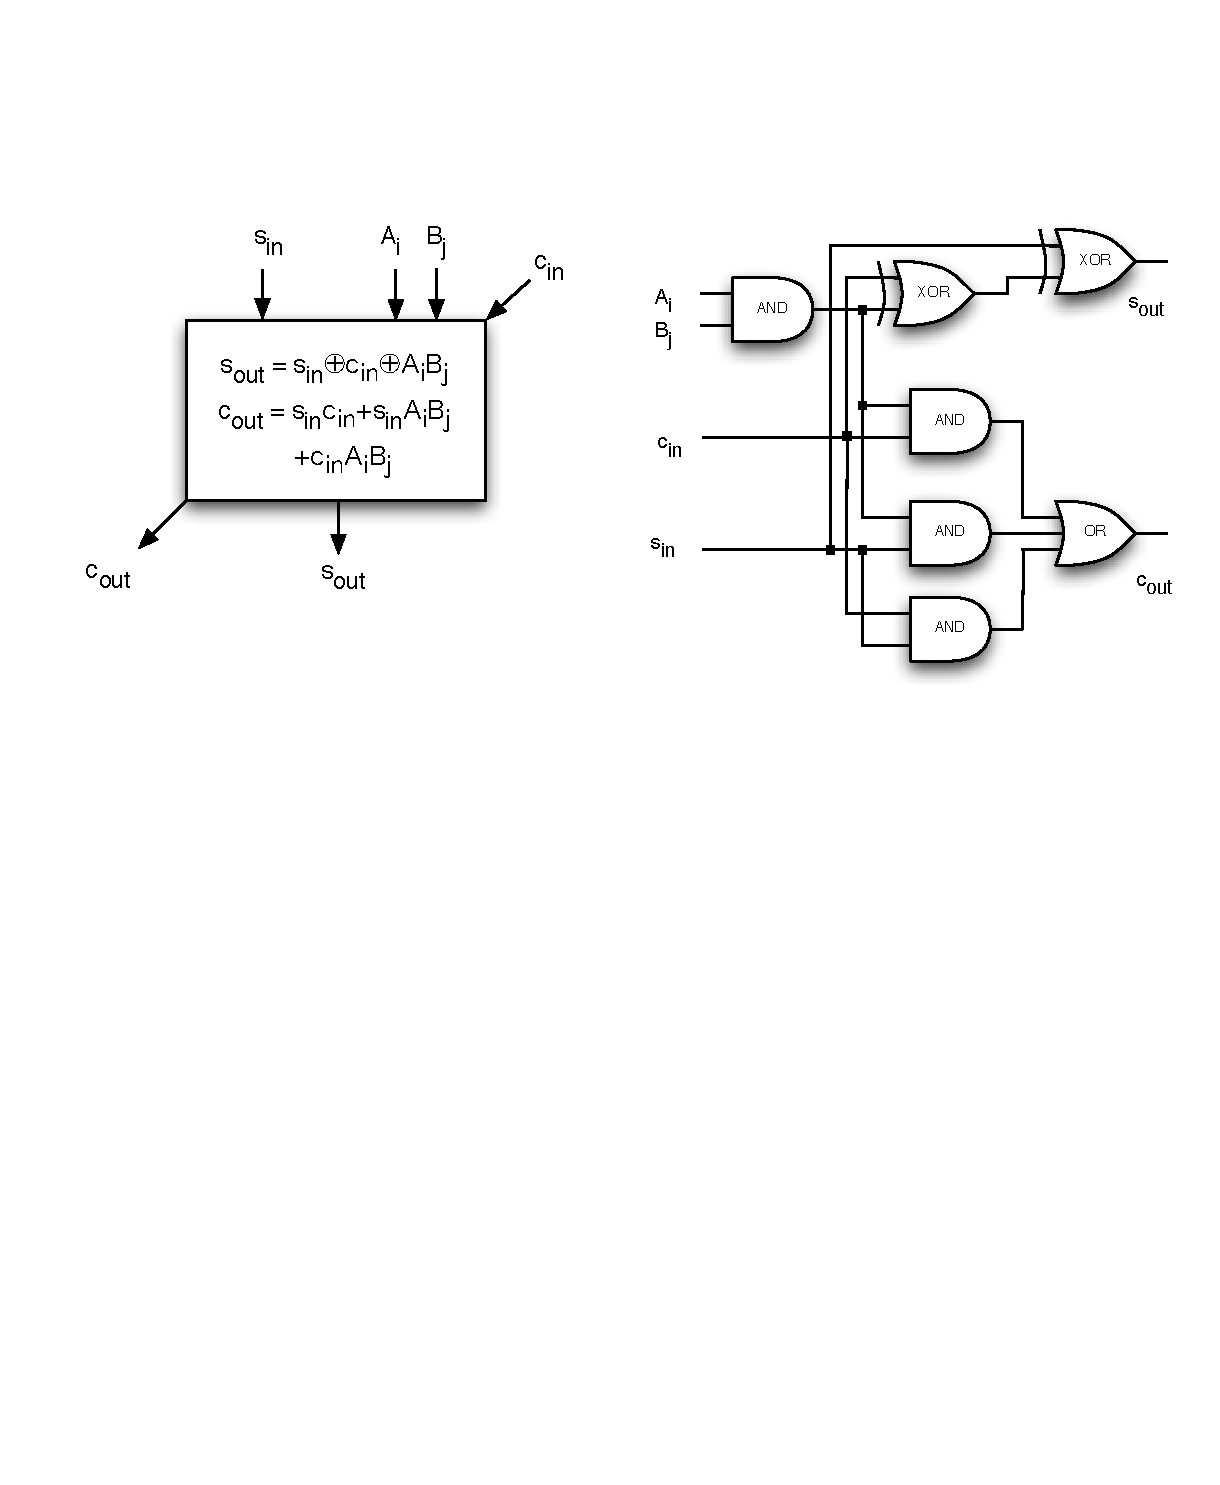
\includegraphics[height=0.4\textheight]{figures/l02/multiplier-1.pdf} \\
		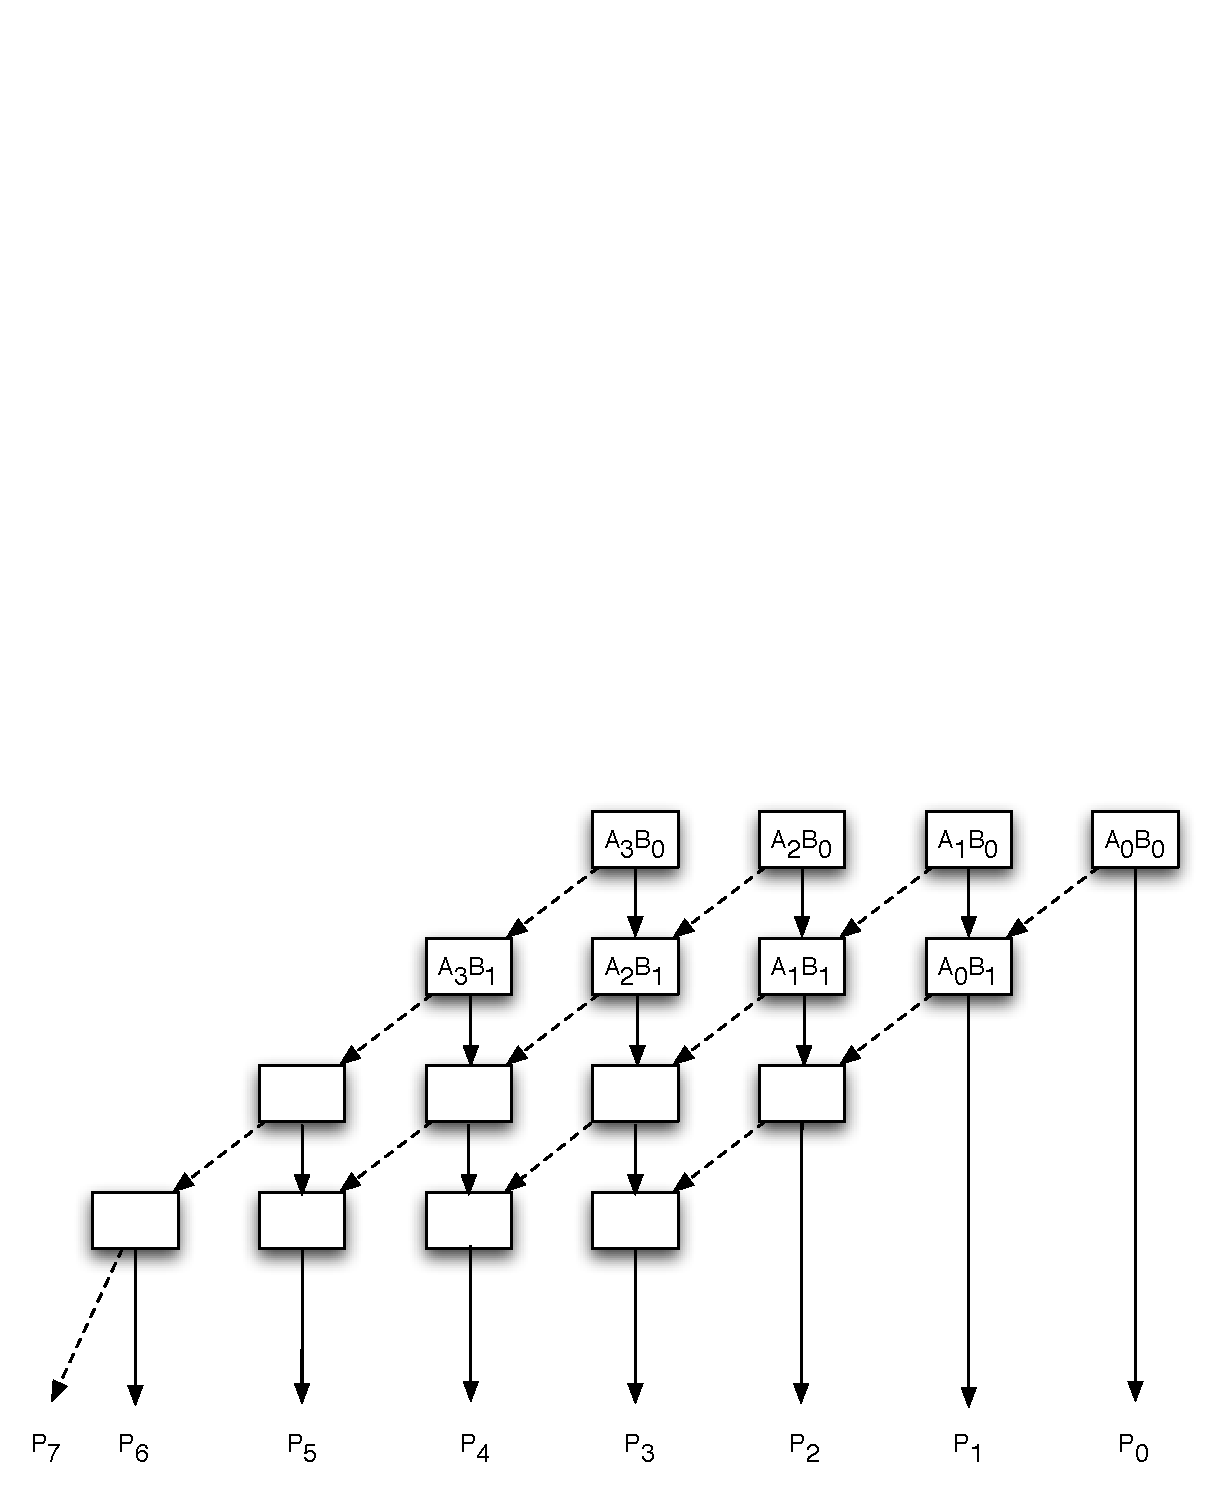
\includegraphics[height=0.4\textheight]{figures/l02/multiplier-2.pdf}
	\end{center}
\end{frame}

\end{document}
